\chapter{Introduction} 

In statistics, we come across collections of probability distributions, such as the normal distribution, Poisson distribution, and binomial distribution. We use these distributions to model random variables in applications, and we refer to them as \emph{statistical models}; precisely, a statistical model is a set of probability distributions. In this thesis, we consider \emph{discrete statistical models} with \emph{finitely many state spaces} \( n + 1 \); we view these models as subsets of the probability simplex \( \Delta_n \coloneqq \left\{ p \in \mathbb{R}^{n + 1} \mid \sum_{k=0}^n p_k = 1 \right\} \), where a distribution \( p \in \Delta_n \) is a point in the probability simplex that assigns probabilities to the states \( 0, \dots, n \).
 
\begin{example}
Say we have a binomial random variable \( X \) with \( n + 1 \) states, then \( p = (p_k)_{k=0}^n = (\binom{n}{k} \theta^k (1-\theta)^{n-k})_{k=0}^n \) computes the probability of observing \( k \) successes in \( n \) trials with success probability \( \theta \in [0,1] \). The set \( \mathcal{M} = \left\{ (\binom{n}{k} \theta^k (1-\theta)^{n-k})_{k=0}^n \mid \theta \in [0,1] \right\} \) is our first example of a discrete statistical model, and it is known as the \emph{binomial model}.

\begin{figure}[H]
    \centering
    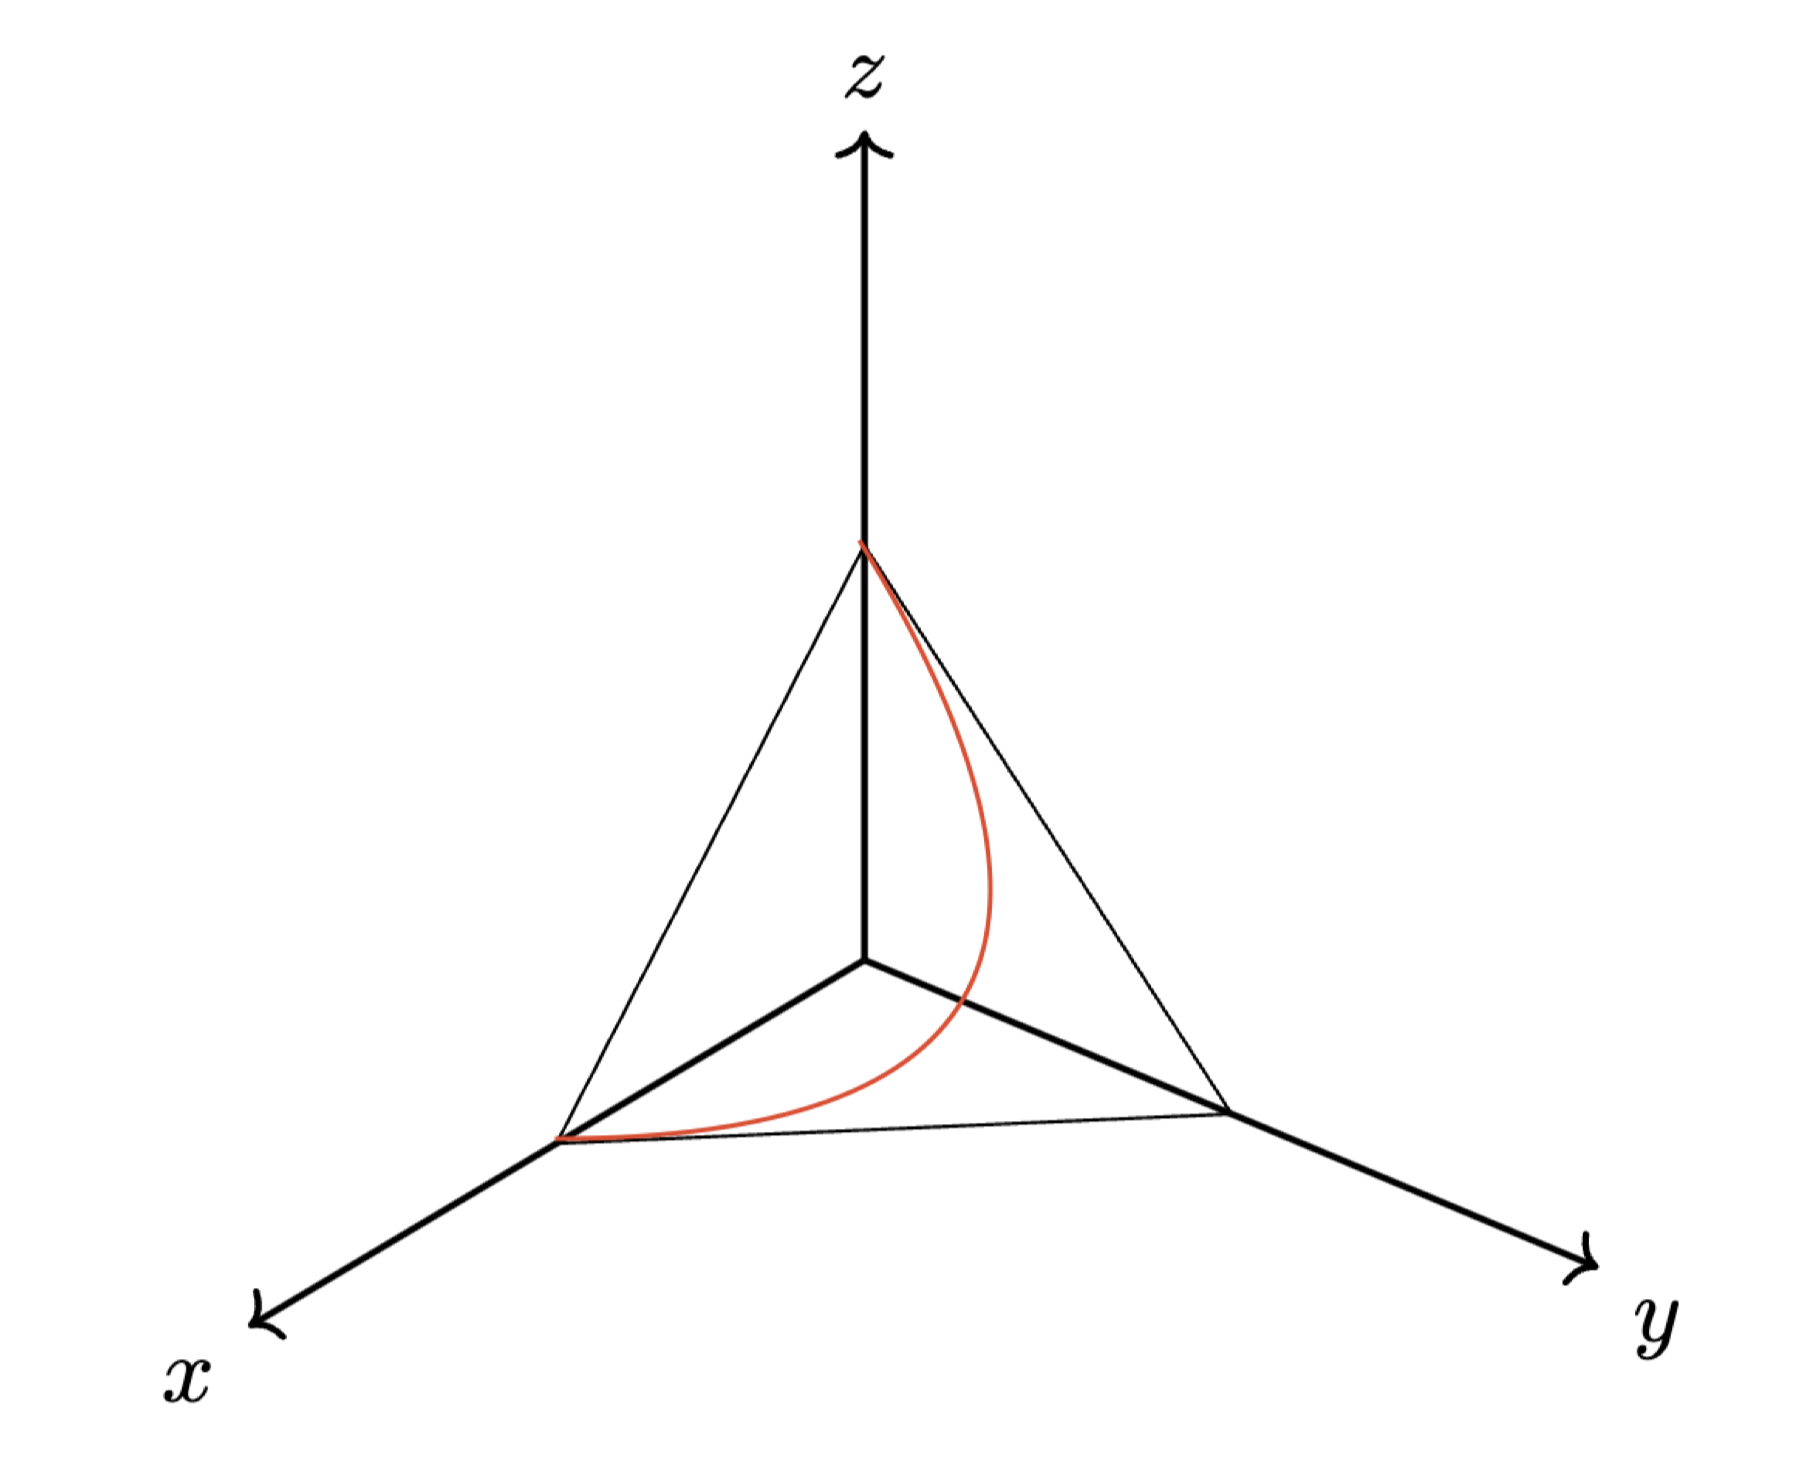
\includegraphics[width=0.43\textwidth]{assets/binom-discrete-model.png}
    \caption{This figure shows the probability simplex \( \Delta_2 \) with the binomial model (red curve). Every point on the curve is a binomial distribution.}
    \label{fig:binom-discrete-model}
\end{figure}
\end{example}

Given a statistical model \( \mathcal{M} \subset \Delta_n \) and data \( u \in \mathbb{N}^{n+1} \), a typical problem in statistics is to find a distribution from a statistical model that best describes the data. ``Best'' can mean a lot of things; in \emph{maximum likelihood estimation}, it refers to finding the distribution that maximizes the probability of observing the data. The mapping
\[
\Phi: \Delta_n \to \mathcal{M}, \quad u \mapsto \hat{p},
\]
that assigns data \( u \) to a distribution \( \hat{p} \in \mathcal{M} \) in the best possible way, in the sense of maximum likelihood estimation, is called the \emph{maximum likelihood estimator (MLE)}. It is characterized by the property that \( \hat{p} \) maximizes for all \( p \in \mathcal{M} \) the log-likelihood function
\[
\ell(p) = \sum_{k=0}^n u_k \log p_k.
\]

We focus on \textbf{{one-dimensional {discrete} {statistical} {models} with rational MLE}}. These are models \( \mathcal{M} \) satisfying 
\begin{itemize}
    \item \( \mathcal{M} = \mathrm{image}(p) \) for some rational map \( p = (p_0, \dots, p_n): I \to \Delta_n \) where \( p_k \) is a rational map, \( I \subset \mathbb{R} \) is a union of closed intervals such that  \( p(\partial I) \subset \partial \Delta_n \);
    \item all the \( n+1 \) coordinates of the maximum likelihood estimator \( \Phi \) are rational functions in the data \( u \).
\end{itemize}

We ask two intriguing questions about these statistical models: (1) which \emph{form} do they take, and (2) can we \emph{classify} them, i.e. can we divide them into easier to understand models? June Huh gave an answer to the first question; he showed that if \( \Phi \) is rational, then each of its coordinates is an alternating product of linear forms with a numerator and denominator of the same degree \cite{huh2013varieties, huh2013maximum, duarte2021discrete}. For the second question, Arthur Bik and Orlando Marigliano provided a framework to classify discrete statistical models with rational MLE by introducing the concept of \emph{fundamental models} and \emph{chipsplitting games} \cite{bik2022classifying}.

This thesis continues the work of Bik and Marigliano. We present their work on how fundamental models serve as the building blocks of statistical models, and whether there are infinitely many fundamental models. As it turns out, they showed that only finitely many fundamental models exist in \( \Delta_n \) for \( n \leq 4 \); we will show this result. The cases \( n \geq 5 \) were left open due to the complexity of the problem. This thesis makes progress for \( n = 5 \) by reducing the number of cases to check from 300,000 to 12,000. Additionally, we present new results on the number of fundamental models in \( \Delta_6 \) with a maximum degree of eleven. The algorithm for solving non-trivial hyperfield linear systems, which drives all the computational work presented, is presented.

This thesis builds upon the work of Bik and Marigliano. We present their findings on how fundamental models act as the building blocks of statistical models and investigate whether infinitely many fundamental models exist. It turns out that only finitely many fundamental models exist in \( \Delta_n \) for \( n \leq 4 \); a result that we will prove using the techniques by Bik and Marigliano. For \( n \geq 5 \), the problem remains open due to the complexity of the problem. This thesis advances the understanding of \( n = 5 \) by reducing the number of cases to check from 300,000 to 12,000. Furthermore, we present new findings on the number of fundamental models in \( \Delta_6 \) with a maximum degree of eleven. Moreover, we describe the algorithm for solving non-trivial hyperfield linear systems that underpins all the computational work discussed in this thesis. 

The outline of this thesis is designed to first introduce the minimum required tools necessary for proving the key results. Once these tools are established, they are applied to prove the main statements. 

The chapters are organized as follows:
\begin{itemize}
    \item Chapter 2 provides a tool to classify statistical models using fundamental models.
    \item Chapter 3 defines chipsplitting games and establishes the connection between fundamental statistical models and fundamental chipsplitting outcomes.
    \item Chapter 4 proves the finiteness of fundamental chipsplitting outcomes with positive support size \( n \leq 3 \) using the Invertibility Criterion.
    \item Chapter 5 proves the case \( n = 4 \) using the \emph{Hyperfield Criterion} and the Invertibility Criterion.
    \item Chapter 6 introduces the final tool, the \emph{Hexagon Criterion}, to show the case \( n = 5 \) using all three tools developed.
    \item Chapter 7 presents novel techniques to reduce the number of cases that need to be analyzed for \( n = 6 \).
    \item Chapter 8 computes the number of fundamental models extending the results of Bik and Marigliano.
    \item Chapter 9 concludes with a discussion on future research directions.
\end{itemize}


We could have opted to collect all the tools first and then apply them collectively to \( n \leq 4 \); however, we believe the current structure is more pedagogical and easier to follow. This approach emphasizes the challenges specific to each case.

The source code for the computations discussed in this thesis is available at \cite{ducrepo}.